

\section{VCAL问题的核心化} \label{KerneliseAlgorithm}
核心化技巧,是指通过多项式时间复杂度的算法将原本的参数化问题实例转化成一个规模更小(参数变小)的新问题实例,
期间需要保证两个问题实例是等价的(其中一个问题实例存在解等价于另外一个存在解) 。
这是固定参数算法(FPT)的设计过程中一个非常重要的技巧。
最直观的角度上看,通过核心化技巧可以缩小问题实例的规模,显然有利于后续的求解。
同时当问题实例已经到不能进一步核心化的状态,
那么可以从这一点上推导出当前实例很多特殊的性质。

本节中的核心化算法时间复杂度是$O(\abs{V} + \abs{E})$,会在每次运行分支算法之前被调用,
以保证在分支算法运行的图中,全$\frac{1}{2}$函数是Primal-$LPVC(G)$问题的唯一最优解($surplus(G) \ge 1$)。
另外,我们要求核心化算法的输入中已经包含了求解当前图的Dual-$LPVC(G)$的网络$W$以及$W$上的最大可行流$f$,
并且算法会构造并输出好基于新图的网络以及相应最大可行流。
这个是我们本节里的核心化算法的目标。

接下来给出具体的算法,其包含两个阶段。

\subsection{核心化算法阶段一}
在本阶段中,算法对输入的图$G$进行收缩,使得全$\frac{1}{2}$函数成为图$G$上Primal-$LPVC(G)$问题的最优解
(根据引理\ref{relationBwtSurplusAndLPVC},即$surplus(G) \ge 0$)。
\vspace{0.5cm}

首先根据\ref{TransformToNetwork}节, 我们可以通过$W$上的最大可行流构造出图$G$上Primal-$LPVC(G)$问题的最优半整数解以及
Dual-$LPVC(G)$问题的最优半整数解,分别用$x$和$y$表示。

从引理\ref{relationBwtVCAndLPVC}上,我们知道存在一个图$G$的最小顶点覆盖包含所有$V^x_1$中的顶点,
并且不包含所有$V^x_0$中的顶点。
因此我们可以首先将图$G$中$V^x_1$里的顶点选进顶点覆盖集合里,
再判断图的剩余部分是否存在最多$k - \abs{V^x_1}$个顶点的顶点覆盖。
同时$V^x_0$中顶点,在$V^x_1$被取走后变成孤立点,也可以被删除,
所以我们从图$G$中删除掉所有$V^x_1$和$V^x_0$中顶点以及与这些顶点相邻的所有边,得到:
\begin{equation*}\begin{aligned}
    &G^* = (V^*, E^*),\;k^* = k - \abs{V^x_1} \\
    &V^* = V^x_{1/2} \\
    &E^* = \{\{u, v\} \in E\;|\;u \in V^*\;and\;v\in V^*\}
\end{aligned}\end{equation*}

我们已经成功将图$G$收缩成了图$G^*$,接下来要考虑如何在快速构造出图$G^*$上Dual-$LPVC(G)$模型的最优解。
因为图$G^*$本质上是图$G$在顶点子集$V^x_{1/2}$上的导出子图,很自然的我们会猜想,
是不是将函数$x,y$定义域收缩为$V^*$和$E^*$后就分别是图$G^*$上Primal-$LPVC(G)$与Dual-$LPVC(G)$的最优解。
接下来,我们对该猜想进行证明。

将函数$x,y$定义域分别限定为$V^*$以及$E^*$,
获得函数$x^*:V^* \rightarrow \mathbb{R}$及$y^*:E^* \rightarrow \mathbb{R}$,
即对任意图$G^*$上的顶点$v$,有$x^*_v=x_v$;对任意图$G^*$上的边$e$,有$y^*_e=y_e$。
\begin{claim}
$x^*, y^*$分别是图$G^*$上Primal-$LPVC(G)$, Dual-$LPVC(G)$的半整数最优解。
\end{claim}
\begin{proof}
因为$x, y$分别是图$G$上Primal-$LPVC(G)$, Dual-$LPVC(G)$的半整数最优解,
显然$x^*, y^*$也应该分别是图$G^*$上Primal-$LPVC(G)$, Dual-$LPVC(G)$的半整数解。
否则在图$G^*$上存在线形规划模型的约束条件不被函数$x^*$(或$y^*$)满足,而该条件在图$G$上也同样不被函数$x$(或$y$)不满足,这与$x$(或$y$)作为最优解冲突。

根据定义可以知道,$x^*$是从$x$中移除掉定义域$V^x_1 \cup V^x_0$后获得的,故$val(x) - \abs{V^x_1} = val(x^*)$。
另外,$y^*$定义域相比$y$移除了与$V^x_1$相邻的边集,即
\begin{equation*} \begin{aligned}
val(y) - val(y^*) & = \sum_{e \in (E \setminus E^*)}{y_e}
\\ & = \sum_{e \in \delta(V^x_1)}{y_e}  \le \sum_{v \in V^x_1}{\sum_{e \in \delta(v)}{y_e}}\le\abs{V^x_1}
\end{aligned}\end{equation*}
结合, $val(y) = val(x)$, 可知$val(y^*) \ge val(x^*)$。

因此$x^*, y^*$分别是图$G^*$上Primal-$LPVC(G)$, Dual-$LPVC(G)$的解,且$val(y^*) \ge val(x^*)$,
根据引理\ref{relationBwtPrimalAndDual}有$x^*, y^*$分别是图$G^*$上Primal-$LPVC(G)$, Dual-$LPVC(G)$的最优解。

证毕。
\end{proof}

比较两个问题实例$(G, k)$和$(G^*, k^*)$,根据引理\ref{relationBwtVCAndLPVC},可以很容易判断他们是等价的。
对于现在新的VCAL上的问题实例$(G^*, k^*)$显然其参数相比于原实例$(G, k)$保持了不变,如下:
\begin{equation*} \begin{aligned}
  \mu(G^*, k^*) &= k^* - vc^*(G^*) \\
                &= (k - \abs{V^x_1}) - (vc^*(G) - \abs{V^x_1}) \\
                &= k - vc^*(G) = \mu(G, k)
\end{aligned} \end{equation*}

对于图$G^*$上求解Dual-$LPVC(G^*)$的网络$W^*$,
因为图$G^*$是原来的图$G$的导出子图,所以根据定义\ref{NetworkDefintion},网络$W^*$显然是原网络$W$的子网络。
同时既然我们已经证明了$y^*$是图$G^*$上Dual-$LPVC(G^*)$模型的最优解,
回顾\ref{TransformToNetwork}节里,Dual-$LPVC$模型的最优解与对应网络最大可行流之间关系,
可以知道将网络$W$的最大可行流$f$定义域限定到子网络$W^*$的边集上便是网络$W^*$的最大可行流。

\subsection{核心化算法阶段二}
因为在上一节中已经将VCAL问题实例$(G, k)$收缩至使得全$\frac{1}{2}$函数是图$G$上Primal-$LPVC(G)$模型的最优解(不保证唯一性),
并且构造出对应的网络$W$的最大流$f$。
接下来在本阶段内,我们会对其问题进行进一步核心化,使得全$\frac{1}{2}$函数成为图$G$上Primal-$LPVC(G)$模型的\textbf{唯一半整数最优解}。
\vspace{0.5cm}

首先,我们给出该阶段算法的基本思路。

如果在当前图$G$满足$surplus(G) = 0$,根据定义可以找到图$G$的某个独立集$S \subseteq V$,使得$surplus(S) = 0$。
构造函数$x':V \rightarrow \mathbb{R}$,如下:
\begin{equation*}
   \begin{cases}
            x'_v =0, & \mbox{对于顶点$v \in S$;}  \\
            x'_v =1, & \mbox{对于顶点$v \in N(S)$;}  \\
            x'_v =\frac{1}{2}, & \mbox{其他。}
          \end{cases}
\end{equation*}
显然$x'$也是$G$的LPVC最优解。
类似上一阶段的做法,我们可以通过将$V^{x'}_1$(即$N(S)$)中顶点选进顶点覆盖集,来将问题实例从$(G,k)$收缩至$(G[V\setminus(S \cup N(S))], k - \abs{N(S)})$。
重复寻找满足条件的独立集$S$,收缩,直到在当前图$G$中$surplus(G) > 0$,则此时已经达到我们核心化的目标,
全$\frac{1}{2}$函数已经是图$G$上Primal-$LPVC(G)$模型的唯一半整数最优解。

观察上述思路,我们发现将算法改进到线性时间复杂度的瓶颈在于如何快速的找到图$G$中满足$surplus(S) = 0$的独立集$S$。
为了突破该瓶颈,我们需要借助网络$W$在最大可行流$f$下的残余图$G_W(f)$。
下面给出若干引理来揭示网络$W$在最大可行流$f$下的残余图$G_W(f)$与满足条件的独立集之间的关系。

回忆网络$W$的构造(定义\ref{NetworkDefintion}),我们将原本图$G$中的每一个顶点$v$,拆分成有向图$G_W$里的$l_v$和$r_v$两个顶点。
为了描述的方便,此处引入几个新的集合的定义,假设$S_W \subseteq V_W$是网络$W$中有向图$G_W$的顶点子集,
令$S_L = \{v\;|\;l_v \in S_W\},S_R = \{v\;|\;r_v \in S_W\}$。
注意此处,$S_W$是网络$W$中的顶点集合,而$S_L, S_R$是图$G$中的顶点集合。
令$L_W = \{l_v \in V_W\}, R_W = \{r_v \in V_W\}$。假设$V' \subseteq V$是图$G$中顶点集合,
另$L_{V'} = \{l_v\in V_W\;|\;v \in V'\},R_{V'} = \{r_v\in V_W\;|\;v \in V'\}$。
注意此处,$L_W, R_W, L_{V'}, R_{V'}$均是网络$W$中的顶点集合。

\begin{lemma} [\cite{iwata2014linear}] \label{residualgraph1}
对于网络$W$里有向图$G_W$的顶点子集$S_W \subseteq (L_W \cup R_W)$, 以下两个条件等价:\footnote{该引理来自于文献\cite{iwata2014linear},但是与之相比本文中我们加强了条件2}
\begin{itemize}
  \item {(1)}在网络$W$的残余图中$G_W(f)$中不存在从$S_W$到$(L_W \cup R_W) \setminus S_W$的边;
  \item {(2)}$N_G[S_L] = S_R$ 并且 $\abs{S_L} = \abs{S_R}$。
\end{itemize}
\end{lemma}
\begin{proof}
  对于当前的图$G$,我们知道$vc^*(G) = \abs{V} / 2$,网络W最大可行流$f$的流量$F=2vc^*(G)=\abs{V}$。
  所以对于图$G$的任意顶点$v \in V$,显然有$f(s, l_v) = f(r_v, t) = 1$。
  假设$V' \subseteq V$,可得流入$L_{V'}$的流量等于流出$R_{V'}$的流量等于$\abs{V'}$。
  回顾残余图的定义,其边有正向反向两种,这里我们也将残余图$G_W(f)$中$S_W$到$(L_W \cup R_W) \setminus S_W$的边分成两个集合,如下:
  \begin{equation*} \begin{aligned}
    & E_L = \{(u, v) \in E_W\;|\;u \in S_W,v \in (L_W \cup R_W) \setminus S_W\} \\
    & E_R = \{(v, u)\;|\;(u, v) \in E_W,f(u, v) > 0,u \in (L_W \cup R_W) \setminus S_W,v \in S_W\}
  \end{aligned} \end{equation*}


  $(1)\rightarrow (2)$: 假设条件(1)成立,等价于$E_L = E_R = \emptyset$。
  由$E_L = \emptyset$,可以知道所有$S_L$中顶点的邻居都在$S_R$中,既$N_G[S_L] \subseteq S_R$。
  由$E_R = \emptyset$,可以知道没有从$S_W$外的顶点有流量流入$S_W \cap R_W$中,所以从$S_W \cap R_W$流出的流量应该小于等于流入$S_W \cap L_W$中的流量,即$\abs{S_R} \le \abs{S_L}$。
  最后,从$S_W \cap L_W$流出的流量显然不可能超过从$R_{N_G[S_L]}$流到汇点t的流量,即$\abs{S_L} \le \abs{N_G[S_L]}$。
  综上有,$\abs{S_L} = \abs{N_G[S_L]} = \abs{S_R}$,再结合前面得到的$N_G[S_L] \subseteq S_R$,可以获得$N_G[S_L] = S_R$。

  $(2)\rightarrow (1)$: 假设$N_G[S_L] = S_R$ 并且 $\abs{S_L} = \abs{S_R}$。
  由于$N_G[S_L] = S_R$,那么$E_L$肯定是空集。
  因为$\abs{S_L} = \abs{S_R}$,那所有流到$S_W \cap R_W$的流量肯定都来自$S_W \cap L_W$,那么也可以得到$E_R$也为空集。故在网络$W$的残余图中$G_W(f)$中不存在从$S_W$到$(L_W \cup R_W) \setminus S_W$的边。

  证毕。
\end{proof}

观察上述引理\ref{residualgraph1},我们发现条件(2)与是“$S_L$是满足surplus值为0的独立集”的弱化条件,
接下来我们对引理\ref{residualgraph1}里的两个条件中都增加约束,来获得更强的结论。

注意上文已经提及,对于图$G$的任意顶点$v \in V$,显然有$f(s, l_v) = c(s, l_v) = f(r_v, t) = f(r_v, t) = 1$。
所以在残余图$G_W(f)$上,顶点$s,t$会构成单独两个非常特殊的强连通分量。
其中强连通分量$\{t\}$会连向所有其他强连通分量;所有其他强连通分量会连向强连通分量$\{s\}$,
而这两个强连通分量毫无意义。
所以,后面我们讨论残余图$G_W(f)$上强连通分量时候会排除掉这两个特殊的顶点。
即,\textbf{实际上讨论的是有向图$G_W(f) \setminus \{s, t\}$上的强连通分量}。


\begin{lemma} [\cite{iwata2014linear}] \label{residualgraph2}
如果网络$W$的流量残余图$G_W(f)$中,有一个尾强连通分量$S_W$满足$S_L \cap S_R = \emptyset$,
那么$S_L$是图$G$中的一个独立集并且$\abs{S_L} = \abs{N_G(S_L)}$。
\end{lemma}
\begin{proof}
$S_W$是$G_W(f)$中一个尾强连通分量,可以推导出$G_W(f)$中不存在从$S_W$到$(L_W \cup R_W) \setminus S_W$的边。
故依据引理\ref{residualgraph1},可以获得$N_G[S_L] = S_R$ 并且 $\abs{S_L} = \abs{S_R}$。
又因为$S_L \cap S_R = \emptyset$,可以得知$N_G(S_L) = N_G[S_L] = S_R$ 并且 $S_L$是图$G$中一个独立集。证毕。
\end{proof}

\begin{lemma} [\cite{iwata2014linear}] \label{residualgraph3}
如果图$G$中存在独立集$T \subseteq V$满足$\abs{T} = \abs{N_G(T)}$,
那么网络$W$在最大可行流$f$下的残余图$G_W(f)$中存在一个尾强连通分量$S_W$满足$S_L \cap S_R = \emptyset$。
\end{lemma}
\begin{proof}
令$T$表示图$G$中满足$\abs{T} = \abs{N_G(T)}$的最小独立集。
构造$S_W = L_T \cup R_{N_G(T)}$,根据定义$S_L = T, S_R = N_G(T)$。
因为$T$是图$G$中满足$\abs{T} = \abs{N_G(T)}$的独立集,
我们可以获得$N_G(T) = N_G[T]$,即$N_G[S_L] = S_R$。
可以进一步整理得引理\ref{residualgraph1}中的条件(2), $N_G[S_L] = S_R$ 并且 $\abs{S_L} = \abs{S_R}$。
故网络$W$在最大可行流$f$下的残余图$G_W(f)$中不存在从$S_W$到$(L_W \cup R_W) \setminus S_W$的边。

假设$S_W$不是网络$W$在最大可行流$f$下的残余图$G_W(f)$中的强连通分量,
则存在$S_W' \subset S_W$使得$G_W(f)$中不存在从$S_W'$到$S_W \setminus S_W'$的边。
又因为之前已经发现$G_W(f)$中不存在从$S_W$到$(L_W \cup R_W) \setminus S_W$的边,
两者结合可以进一步发现$G_W(f)$中不存在从$S_W'$到$(L_W \cup R_W) \setminus S_W'$的边。
根据引理\ref{residualgraph2},可以发现$S_L'$是图$G$中的一个独立集并且$\abs{S_L'} = \abs{N_G(S_L')}$。
因为$S_W'$是$S_W$的真子集,故$S_L' \subset S_L = T$,这与T是满足$\abs{T} = \abs{N_G(T)}$的最小独立集矛盾。
故假设不成立,$S_W$是网络$W$的残余图$G_W(f)$中的强连通分量。

综上,我们构造的顶点集合$S_W$是网络$W$的残余图$G_W(f)$中的尾强连通分量,且满足$S_L \cap S_R = \emptyset$。

证毕。
\end{proof}

引理\ref{residualgraph2}和引理\ref{residualgraph3},为我们提供了寻找图$G$中满足$surplus$值为0的独立集的方法。
当我们从残余图$G_W(f)$中找到一个尾强连通分量$S_W$满足$S_L \cap S_R = \emptyset$,
则可以判断$S_L$是图$G$的独立集,且满足$surplus(S_L) = 0$。
通过将$N(S_L)$中顶点选进顶点覆盖集,可以获得新的VCAL问题实例如下,
\[(G' \leftarrow G \setminus (S_L \cup N(S_L)),\; k' \leftarrow k - \abs{N(S_L)})\]
对于求解图$G'$上Dual-$LPVC(G')$问题的网络$W'$,同理于上一阶段的证明,我们知道网络$W'$是网络$W$的子网络,
并且网络$W'$的最大可行流$f'$,可以通过将原网络$W$的最大可行流$f$定义域缩小获得。
现在剩下的唯一的问题就是,当前我们每一次找到一个满足盈余值为0的独立集,
就需要重构一遍残余图,重新求解一次强连通分量。
我们希望可以进一步优化,使得只求一次残余图的强连通分量便可以找出所有满足条件的独立集。
为了解决该问题,我们需要分析当把某个顶点集$N(S_L)$选进当前顶点覆盖集后,新的网络最大流残余图$G_{W'}(f')$与之前的残余图$G_W(f)$之间关系。

为了描述方便,令$T = S_L$,则$S_W = L_T \cup R_{N_G(T)}$。
对比网络$W$与网络$W'$发现,除了移除顶点集合$L_T \cup R_{N_G(T)}$,还移除了顶点集合$L_{N_G(T)} \cup R_T$。
如下图\ref{fig:mesh1}当我们从残余图中找到尾强连通分量$\{l_a, l_b, r_c, r_d\}$符合引理\ref{residualgraph2},
此时我们计划从图$G$移除顶点$a, b, c, d$, 则对应回网络$W$中除了上述尾强连通分量,还移除了另外4个顶点。
实际上我们不需要重新计算新网络的残余图强连通分量,因为顶点集合$\{l_c, l_d, r_a, r_b\}$在原残余图中对应着一个头强连通分量。
后续给出断言\ref{residualgraph4}并证明该结论。

\begin{figure}[h]
    \centering
    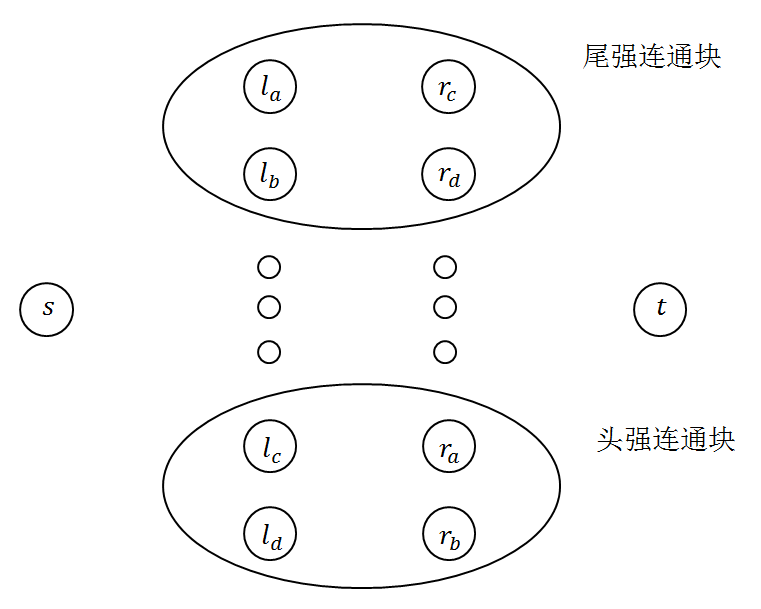
\includegraphics[width=0.65\textwidth]{eps/1.png}
    \caption{残余图中尾强连通分量与对应的头强连通分量}
    \label{fig:mesh1}
\end{figure}

\begin{claim} \label{residualgraph4}
在残余图$G_W(f)$中没有边从顶点集合$(L_W \cup R_W) \setminus (L_{N_G(T)} \cup R_T)$到顶点集合$L_{N_G(T)} \cup R_T$中。
\end{claim}
\begin{proof}
首先我们将残余图$G_W(f)$中
从顶点集合$L_{N_G(T)} \cup R_T$到顶点集合$(L_W \cup R_W) \setminus (L_{N_G(T)} \cup R_T)$中边分成两个集合,
注意在网络$W$中,排除$s, t$后,只有从$L_W$到$R_W$的边。
  \begin{equation*} \begin{aligned}
    & E_L = \{(u, v) \in E_W\;|\;u \in L_W \setminus L_{N_G(T)},v \in R_T\} \\
    & E_R = \{(v, u)\;|\;(u, v) \in E_W,f(u, v) > 0,u \in L_{N_G(T)},v \in R_W \setminus R_T\}
  \end{aligned} \end{equation*}

回顾定义\ref{NetworkDefintion},显然$E_L$为空集。
同时由于$\abs{R_T} = \abs{L_{N_G(T)}}$,且$E_L$为空,
所以所有从集合$L_{N_G(T)}$流出的流量都会流入集合$R_T$中,
因此$E_R$也是空集。

故,$E_L = E_R = \emptyset$,证毕。
\end{proof}



对于残余图$G_W(f)$的所有强连通分量,他们之间构成了拓扑关系。
而新的残余图$G_{W'}(f')$与之对比,移除掉的强连通分量要不就在拓扑关系的顶端(没有外部边可以到达顶点集合$L_{N_G(T)} \cup R_T$中)
要不就在拓扑关系的末端(顶点集合$L_T \cup R_{N_G(T)}$是一个尾强连通分量),
而对于剩余强连通分量,强连通性以及拓扑关系都没有受到影响!
因此只需要在求出残余图$G_W(f)$的所有强连通分量之后,利用逆拓扑顺序遍历每一个强连通分量$S_W$,
检查该强连通分量是否不存在未被标记移除的后代以及是否满足$S_L \cap S_R = \emptyset$,
如果两个条件都成立,则将顶点集合$L_T \cup R_{N_G(T)}$与顶点集合$L_T \cup R_{N_G(T)}$中的强连通分量都标记为移除即可。


至此我们给出了核心化算法阶段二的所有证明,下面分析时间复杂度。
在整个核心化算法阶段二,其中我们只需要构造一个残余图,求出该残余图的所有强连通分量,最后逆拓扑顺序遍历这些强连通分量。
显然每个步骤都是可以做到线性时间复杂度的,故整体时间复杂度为$O(\abs{V} + \abs{E})$。

\subsection{完整核心化算法}

伪代码详见Algorithm 1。

其中,我们将VCAL问题实例以及预先构造好的网络及其最大流作为输入,并且在核心化的过程中也将新图对应的网络及其最大流构造好并输出。


\begin{algorithm} 
\caption{完整核心化算法}
\begin{algorithmic}[1] 
\Require VCAL问题实例$(G,k)$, 图$G$对应的网络$W$及其最大流$f$
\Ensure  核心化后的VCAL问题实例$(G',k')$,图$G'$对应的网络$W'$及其最大流$f'$,被取进顶点覆盖的顶点集合$S_1$,
        ,被排除出顶点覆盖的顶点集合$S_0$
\algrule
\Function{Kernelise}{$G, k, W, f$}
    \State $S_0 \gets \emptyset$
    \State $S_1 \gets \emptyset$
    \State \Comment 核心化算法阶段一
    \State 根据网络$W$在最大可行流$f$,构造图$G$的Primal-$LPVC(G)$最优解$x$

    \State $G_1 \gets G[V^x_{1/2}],\;k_1 \gets k - \abs{V^x_1}$
    \State $S_1 \gets S_1 \cup V^x_1$
    \State $S_0 \gets S_0 \cup V^x_0$
    \State $W_1 \gets \text{从网络$W$中移除顶点集合}\{l_v, r_v | v \in V^x_1 \cup V^x_0\}\text{以及相关边}$
    \State $f_1 \gets \text{将流量函数$f$定义域限定到网络$W'$的边集上}$

    \State \Comment 核心化算法阶段二
    \State 构造网络$W_1$在最大可行流$f_1$下的流量残余图$G_{W_1}(f_1)$
    \State $K \gets \text{求解图$G_{W_1}(f_1) \setminus \{s, t\}$的所有强连通分量}$

    \For {按逆拓扑顺序遍历K中每一个强连通分量$T\in K$}
        \If {强连通分量$T$不存在未被标记的后代\; \textbf{and}\;$\{v\;|\;l_v \in T, r_v \in T\} = \emptyset$}
            \State $S_0 \gets S_0 \cup \{v\;|\;l_v \in T\}$
            \State $S_1 \gets S_1 \cup \{v\;|\;r_v \in T\}$
            \State 标记强连通分量T
        \EndIf
    \EndFor
    \State $G_2 \gets G \setminus (S_0 \cup S_1),\;k_2 \gets k - \abs{S_1}$
    \State $W_2 \gets \text{从网络$W$中移除顶点集合}\{l_v, r_v | v \in S_1 \cup S_0\}\text{以及相关边}$
    \State $f_2 \gets \text{将流量函数$f$定义域限定到网络$W_2$的边集上}$

    \State \Return $(G_2, k_2, W_2, f_2, S_1, S_0)$
\EndFunction
\end{algorithmic}
\end{algorithm} 